\documentclass[11pt]{amsart}
\usepackage[margin=1in]{geometry}                % See geometry.pdf to learn the layout options. There are lots.
\geometry{letterpaper}                   % ... or a4paper or a5paper or ... 
%\geometry{landscape}                % Activate for for rotated page geometry
%\usepackage[parfill]{parskip}    % Activate to begin paragraphs with an empty line rather than an indent
\usepackage{graphicx}
\usepackage{amssymb}
\usepackage{epstopdf}
\DeclareGraphicsRule{.tif}{png}{.png}{`convert #1 `dirname #1`/`basename #1 .tif`.png}

\title{Math 228b, Spring 2014, homework 1}
\author{Jake Edman}
\date{}                                           % Activate to display a given date or no date

\begin{document}
\maketitle
\section{solve $u_t = u_{xx}$ on [0,1] with I.C. $u(x,0)= \sin(\pi x)$}
\subsection{$h=k=1/10$}
Figure \ref{u1} depicts the solution at $t=1$.  This solution is clearly very bad, and unstable. Heat should diffuse out along the domain, away from the initial maximum at $x=0.5$, and because there are no sources or sinks in the domain, it should simply flatten out to zero over time, and never become negative.  Additionally, the solution should be symmetrical along the x axis; the initial condition and boundary conditions are symmetric, and there are no sources or sinks to break the symmetry. The solution depicted in figure \ref{u1} changes sign as we move along the x axis, and is not symmetric, which must arise from  numerical instability. Instability is expected; in class, we showed that this scheme is stable for $\lambda \equiv \frac{k}{h^2} \le \frac{1}{2}$, and in this case $\lambda = 10$. 

\begin{figure}[t]
\begin{center} 
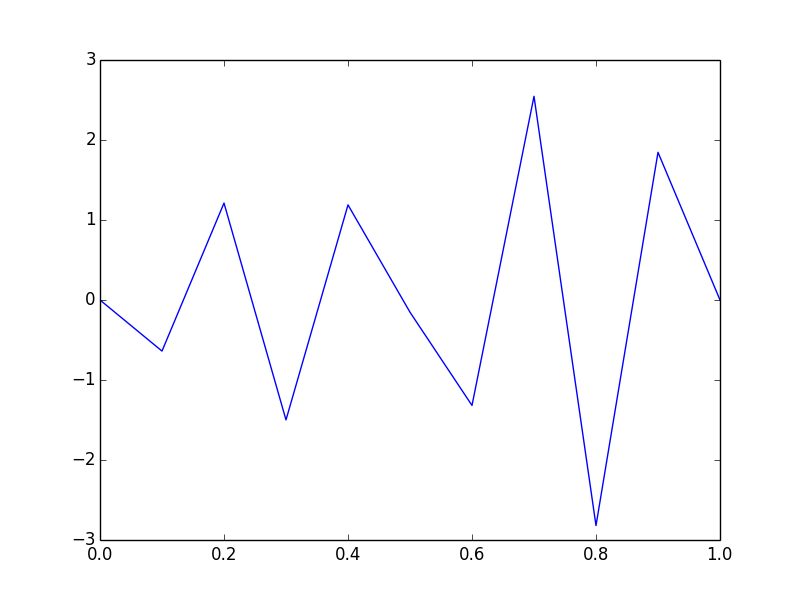
\includegraphics[width=5in,angle=0]{u1.pdf}
\caption{The solution to $u_t = u_{xx}$ with  $h=k=1/10$ }
\label{u1} 
\end{center}
\end{figure}
  
\subsection{$h=1/10$, $k=1/200$}
The solid blue line in figure \ref{u2} depicts the solution at $t=1$. Unlike the solution depicted in figure \ref{u1}, this solution appears stable, because it is smooth, nonnegative, and symmetric. We expect stability, because $\lambda = 1/2$ in this case. 

\begin{figure}[t]
\begin{center} 
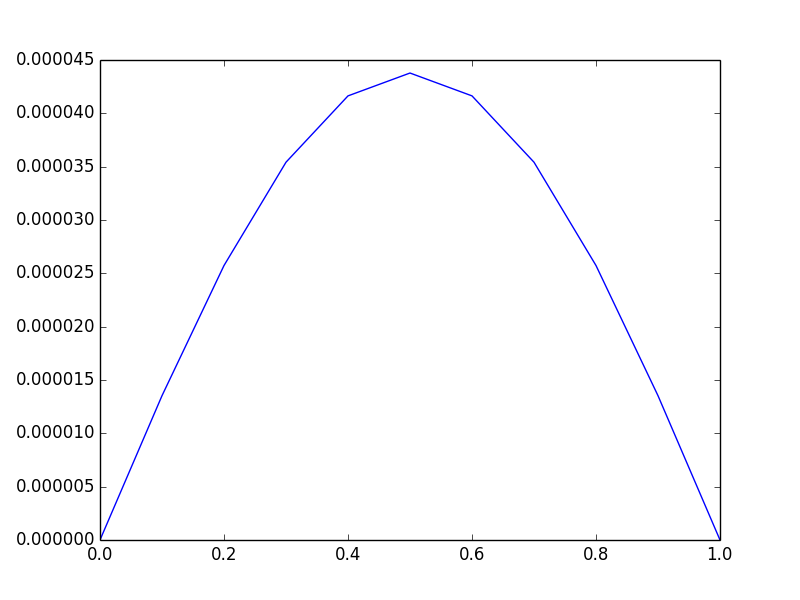
\includegraphics[width=5in,angle=0]{u2.pdf}
\caption{The solution to $u_t = u_{xx}$ with  $h=k=1/10$ }
\label{u2} 
\end{center}
\end{figure}

\subsection{$\lambda = 1/6$} 
The dashed green line in figure \ref{u2} depicts the solution at $t=1$ for $\lambda =1/6$. This solution is clearly different than the one given by $\lambda =1/2$, but is it `better'? 

In class, we showed that truncation error is minimized for $\lambda = 1/6$;  the truncation error is defined as $\tau^k = u^{k} - u^{exact}$ where the superscript $u^k$ refer to the solution on a grid defined by time discretization $k$, and $u^{exact}$ is the exact solution. In this case, we do not have the exact solution, but we can effectively solve for it by using multiple mesh refinements. Assuming the truncation error can be related to the discretization raised to some exponent $r$, such that $\tau^k = Ck^r$, where C is a constant, we can write  
\begin{eqnarray} 
Ck_1^r= u^{k_1} - u^{exact}\\
Ck_2^r = u^{k_2} - u^{exact}\\
Ck_3^r = u^{k_3} - u^{exact}
\end{eqnarray} 
We can solve this system for $r$, the order of convergence, and approximate the exact solution if we choose grids such that $k_3/k_2 = k_2/k_1 =$ constant.

\section{Comparison with exact solution for  I.C. $u(x,0)= \sin(\pi x)$} 

\section{Comparison with exact solution for  I.C. $u(x,0)= x(1-x)$} 

\section{Consider $u_t = \alpha u_{xx}$ on [0,1] with I.C. $u(x,0)= \sin(\pi x)$, where $\alpha$ is a constant. }


\section{Consider $u_t = \alpha(x) u_{xx}$ on [0,1] with I.C. $u(x,0)= \sin(\pi x)$ }


\end{document}  